
\subsubsection{KW46: 15.11.2021 bis 21.11.2021}
\begin{quote}
	\subsubsection*{Arbeit in der Schule}
	Der Ghost Charakter wurde eingefügt, welche ein dynamischer Gegner ist. Der Ghost bewegt sich in einer bestimmten Umgebung und schaut ob er den Charakter in seiner Point of View hat. 
	\subsubsection*{Arbeit außerhalb der Schule}
	Ich konnte in GIT meine Arbeit nicht speichern, da ein Fehler auftauchte.
	Ich habe im Internet recherchiert und in einem Beitrag gelesen, dass man auf Git nicht mehr als 2GB Daten hochladen soll, da sonst Probleme auftauchen könnten. Doch unsere Repository war ca. 4Gb groß. Nachdem wir die unwichtigen Dateien gelöscht haben und ich die Repository nochmals geclont habe, hat alles wieder funktioniert. 
	
	\begin{figure}
		\centering
		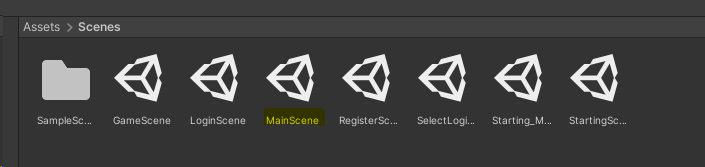
\includegraphics[width=0.7\linewidth]{img/SemihSoenmez_IMG/KW47_unity_scenes2}
		\caption{}
		\label{fig:kw47unityscenes2}
	\end{figure}
\end{quote}
